\chapter{\IfLanguageName{dutch}{Stand van zaken}{State of the art}}%
\label{ch:stand-van-zaken}

% Tip: Begin elk hoofdstuk met een paragraaf inleiding die beschrijft hoe
% dit hoofdstuk past binnen het geheel van de bachelorproef. Geef in het
% bijzonder aan wat de link is met het vorige en volgende hoofdstuk.

% Pas na deze inleidende paragraaf komt de eerste sectiehoofding.

%Dit hoofdstuk bevat je literatuurstudie. De inhoud gaat verder op de inleiding, maar zal het onderwerp van de bachelorproef *diepgaand* uitspitten. De bedoeling is dat de lezer na lezing van dit hoofdstuk helemaal op de hoogte is van de huidige stand van zaken (state-of-the-art) in het onderzoeksdomein. Iemand die niet vertrouwd is met het onderwerp, weet nu voldoende om de rest van het verhaal te kunnen volgen, zonder dat die er nog andere informatie moet over opzoeken \autocite{Pollefliet2011}.

%Je verwijst bij elke bewering die je doet, vakterm die je introduceert, enz.\ naar je bronnen. In \LaTeX{} kan dat met het commando \texttt{$\backslash${textcite\{\}}} of \texttt{$\backslash${autocite\{\}}}. Als argument van het commando geef je de ``sleutel'' van een ``record'' in een bibliografische databank in het Bib\LaTeX{}-formaat (een tekstbestand). Als je expliciet naar de auteur verwijst in de zin (narratieve referentie), gebruik je \texttt{$\backslash${}textcite\{\}}. Soms is de auteursnaam niet expliciet een onderdeel van de zin, dan gebruik je \texttt{$\backslash${}autocite\{\}} (referentie tussen haakjes). Dit gebruik je bv.~bij een citaat, of om in het bijschrift van een overgenomen afbeelding, broncode, tabel, enz. te verwijzen naar de bron. In de volgende paragraaf een voorbeeld van elk.

%\textcite{Knuth1998} schreef een van de standaardwerken over sorteer- en zoekalgoritmen. Experten zijn het erover eens dat cloud computing een interessante opportuniteit vormen, zowel voor gebruikers als voor dienstverleners op vlak van informatietechnologie~\autocite{Creeger2009}.

%Let er ook op: het \texttt{cite}-commando voor de punt, dus binnen de zin. Je verwijst meteen naar een bron in de eerste zin die erop gebaseerd is, dus niet pas op het einde van een paragraaf.

%\lipsum[7-20]

In de stand van zaken wordt er informatie gegeven over de verschillende onderwerpen omtrent de extractie van informatie uit documenten met behulp van artificiële intelligentie. Allereest wordt er toegelicht wat information extraction precies inhoudt. Daarna wordt er uitleg gegeven over Named Entity Recognition, wat een onderdeel is van Information Extraction. Verder wordt er uitgelegd hoe dit gerealiseerd kan worden aan de hand van artificiële intelligentie en deep learning. Tot slot is er nog uitleg over verschillende soorten libraries, die vaak een grote rol spelen in het ontwikkelen van zulke toepassingen.

\section{Master data en master data management}

\textcite{loshin2010master} definieert master data als belangrijke bedrijfsobjecten die gebruikt worden in verschillende applicaties binnen de organisatie, zoals klanten, leveranciers, werknemers, producten \ldots. Master data bestaat doorgaands in meer dan één bepaald deel van het bedrijf, zo kan een klant bijvoorbeeld zowel in de boekhouding als in de verkoopafdeling voorkomen. Naast dat master data cruciaal is voor de werking van de systemen binnen een bedrijf, kunnen de catergorieën van master data ook gebruikt worden om raporten en inzichten te maken zoals bijvoorbeeld: verkopen per klant per regio \autocite{loshin2010master}.

Master data management omvat het ontwikkelen van één bron van waarheid voor de master data van een bedrijf. Om dit te bereiken wordt de data gede-dupliceerd, afgestemd op elkaar en verrijkt om een consistente en betrouwbare bron te worden \autocite{silvola2011managing}. 

Een doeleinde waar master data management wordt toegepast is Enterprise Resource Plannning (ERP). ERP volgt een aanpak waarbij Bedrijfsprocessen centraal staan en intergreert master data langs deze processen. Dit zorgt ervoor dat alle processen, maar vooral de master data centraal wordt beheerd en dat dit consistent blijft \autocite{maedche2010erp}.

\section{SAP}

SAP is een van de grootste ontwikkelaars van bedrijfsmanagement-software. SAP is opgestart in 1972 door 5 personen en nu een grote multinational met meer dan 105.000 werknemers. SAP is begonnen met het maken van Enterprise Resource Planning (ERP) software, met als voriges versies: SAP R/2 en SAP R/3 en neemt ERP naar een nieuw niveau door SAP S/4HANA. In deze versie gebruiken ze nieuwe in-memory technologieën om grote aantallen data te kunnen verwerken, ook gebruiken ze nieuwe zaken zoals: cloud, AI en machine learning om de workflow van klanten verder te versnellen \autocite{SAP} 

\section{Enterprise Resource Planning}

Enterprise Resource Planning (ERP) is volgens \textcite{SAPERP} een softwaresysteem dat bedrijven helpt om hun zaak te draaien en processen te ondersteunen. In het kort helpt een ERP systeem om efficiënt grote processen zoals: Boekhouding, HR, productie\ldots. samen te brengen en te ondersteunen. Dit zorgt ervoor dat alle data centraal via 1 systeem wordt beheerd en alles simpel doorgegeven kan worden tussen de verschillende diensten. \textcite{SAPERP} geeft dan ook aan dat de moderne ERP-systemen alles behalve een simpel stukje software zijn, maar tegenwoordig via de cloud en met de nieuwste technologieën worden geleverd.

\begin{figure}[h]
  \centering
  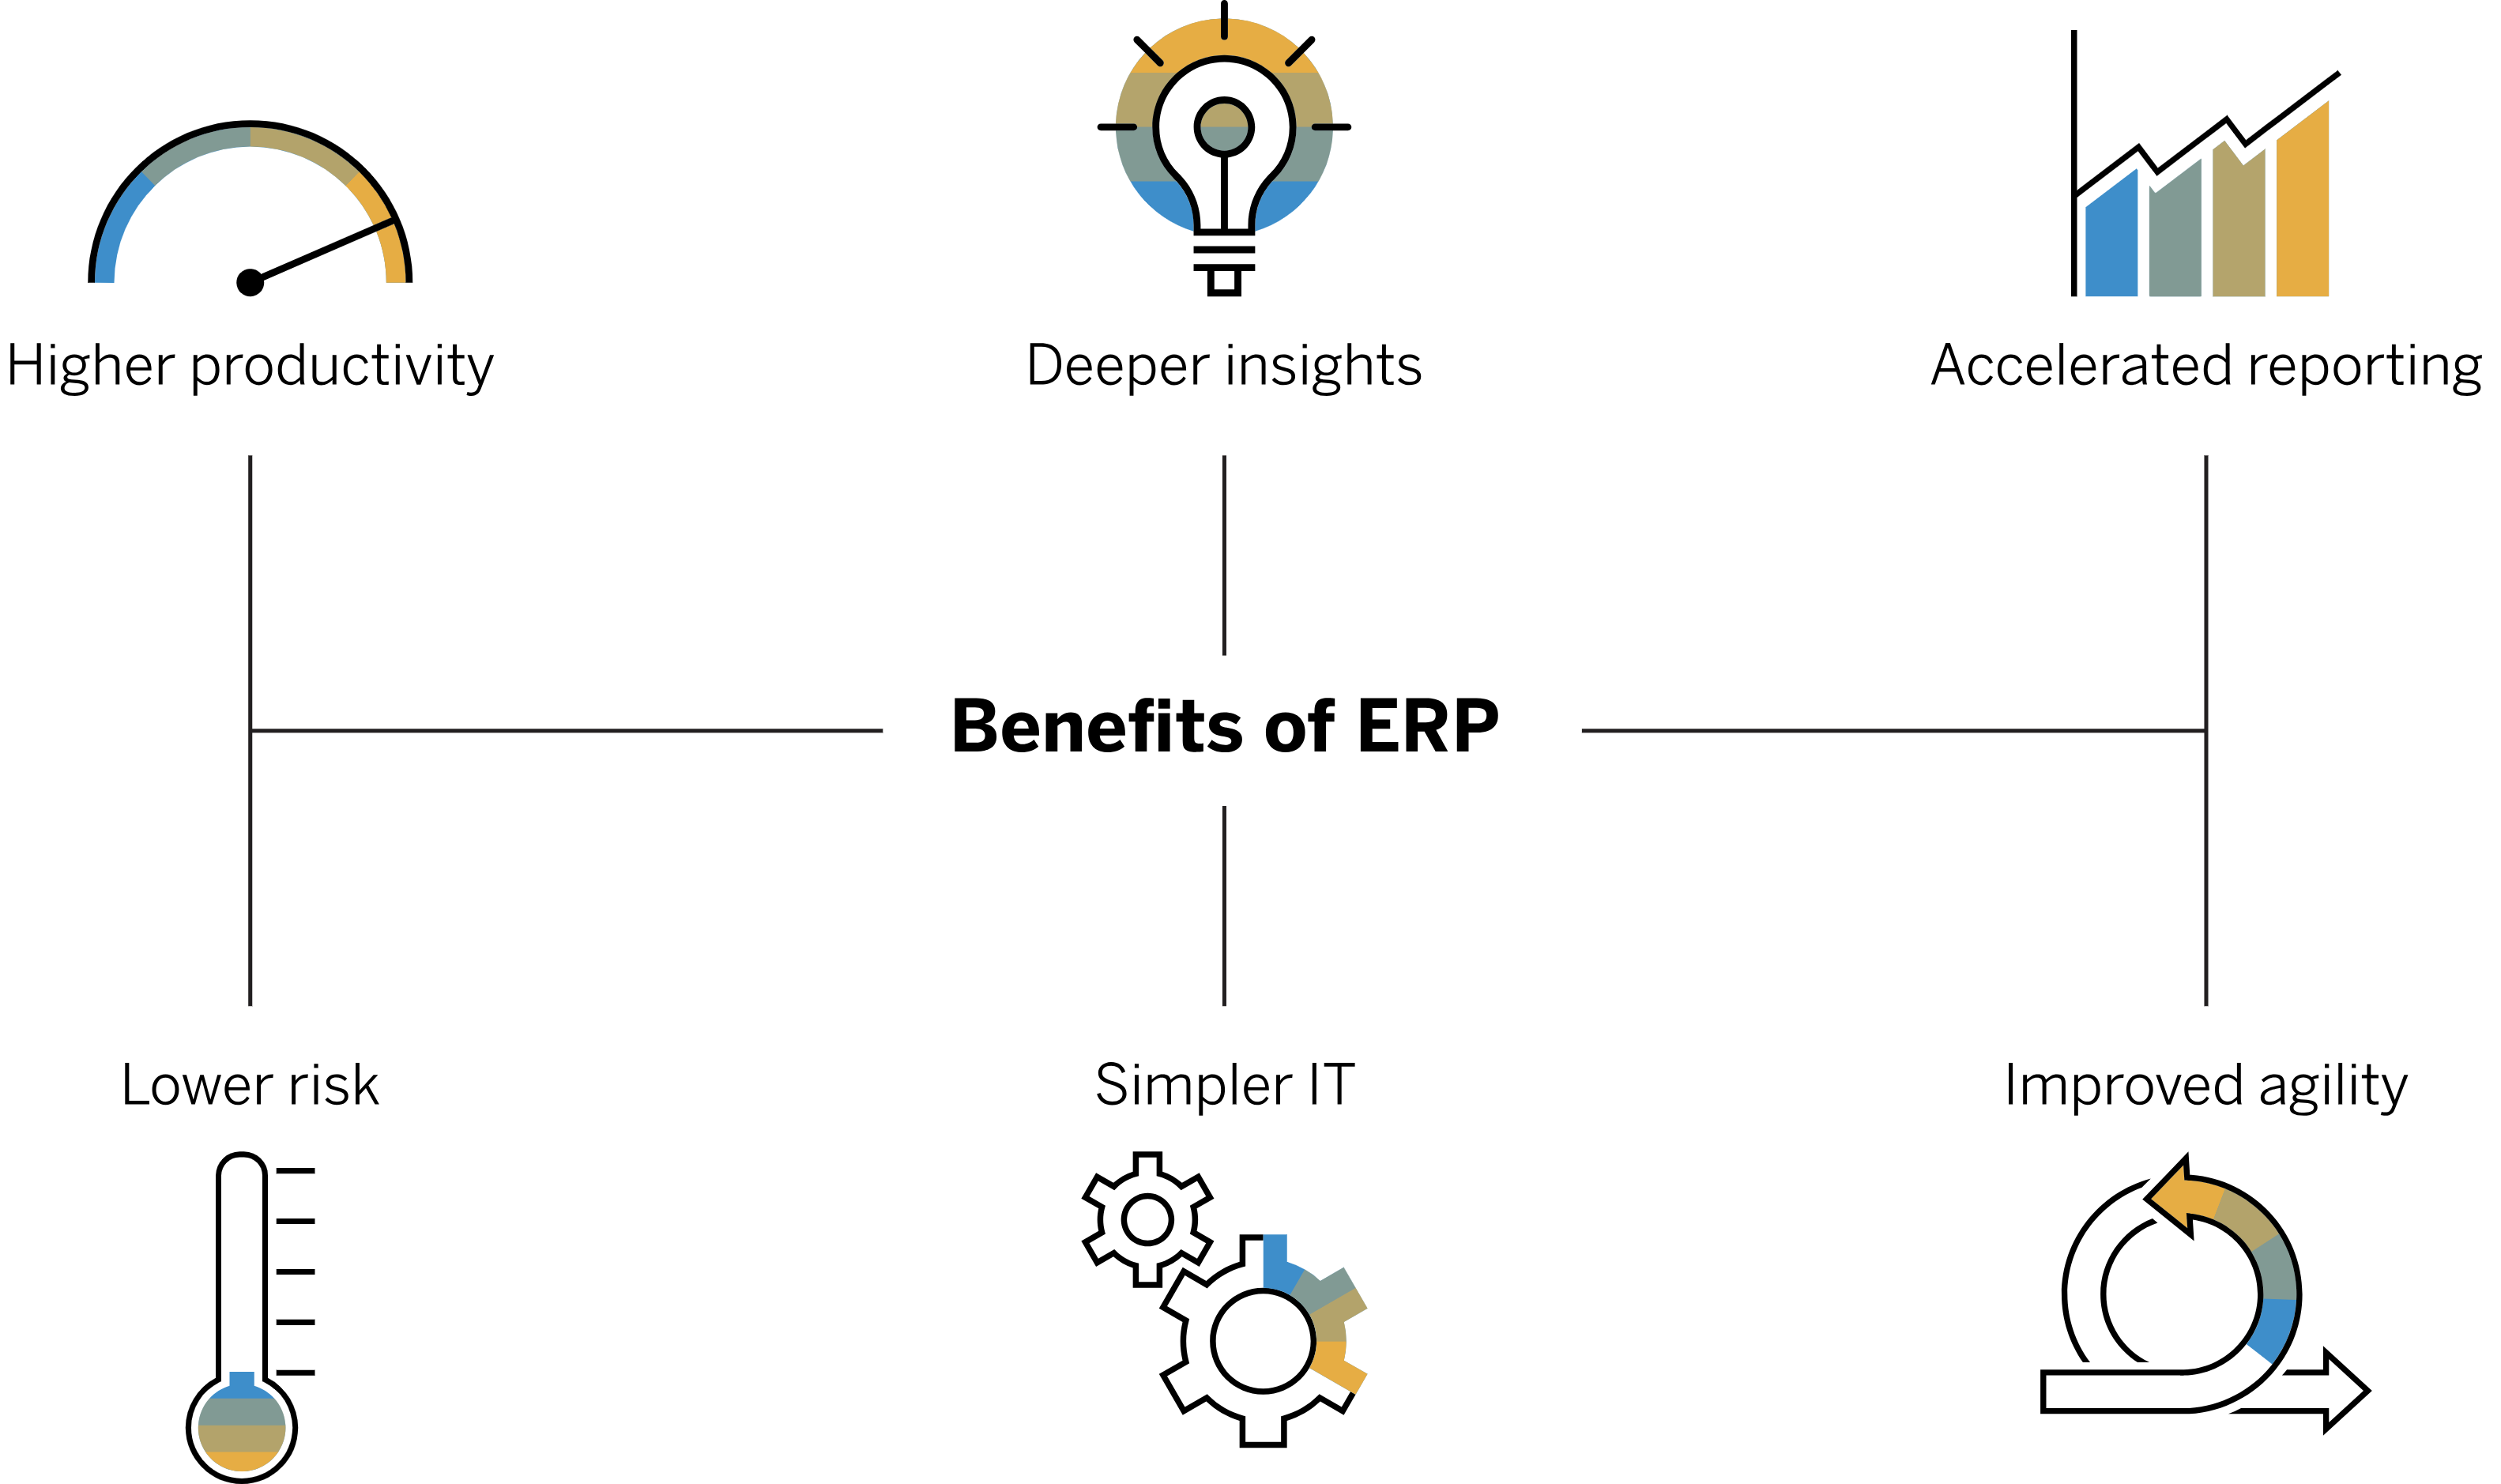
\includegraphics[width=.8\textwidth]{./graphics/erp-benefits}
  \caption{\label{fig:benefitserp}Voordelen van een ERP-systeem \autocite{SAPERP}}
\end{figure}

Volgens \textcite{SAPERP} zijn er dan ook verschillende voordelen aan het gebruiken van een ERP-systeem:
\begin{itemize}
  \item \textbf{Hogere productiviteit:} Bedrijfsprocessen automatiseren en optimaliseren om iedereen meer te laten doen met minder middelen.
  \item \textbf{Beter inzicht:} Een enkele opslag van data, een bron van data die antwoord kan geven op alle bedrijfsvragen.
  \item \textbf{Snellere rapportage:} Versnelde rapportage en gemakkelijk resultaten delen. Sneller actie nemen en prestatie verbeteren.
  \item \textbf{Minder risico:} Verzeker dat het bedrijf regelementair in orde is en risico velagen.
  \item \textbf{Simplere IT:} Geef IT een gemakkelijkere manier om te werken door alles te integreren in een ERP-systeem.
  \item \textbf{Meer flexibiliteit:} Met efficiënte operaties en directe toegang tot realtime gegevens kan er sneller nieuwe kansen identificeren en erop reageren.
\end{itemize}
\section{Information Extraction}

Information Extraction(IE) is een manier om tekst te doorzoeken met als doel belanghebbende informatie te vinden voor bepaalde doeleinden. Het omvangt meer dan enkel en alleen trefwoorden te zoeken in de tekst, maar de doelstellingen blijven achter bij het probleem van tekstbegrip, waarbij we proberen alle informatie in een tekst vast te leggen, samen met de intentie van de schrijver \autocite{hobbs2010}. Volgens \textcite{Freitag2000} is IE het probleem van het samenvatten van essentiële details die specefiek zijn voor een bepaald documenten. Een apparte samenvatting gemaakt door een computerprogramma zal een template aanhouden die bepaalde velden invult aan de hand van de tekst uit het document.

IE ligt tussen twee andere methodes van tekstverwerking, namelijk information retrieval en natuurlijke taalverwerking. IE kan worden beschouwd als een soort goedkoop, gericht begrijpen van natuurlijke taal. IE gaat uit van een verzameling documenten, waarin elk document namen en gebeurtenissen beschrijft die op elkaar lijken, maar waar de details verschillen. Voor een IE-taak wordt er een sjabloon voorzien die beschrijft wat voor informatie er in het document staat \autocite{Freitag2000}

\section{Natural language processing}

\textcite{allen2003natural} zegt dat natural language processing(NLP) verwijst naar computersystemen die menselijke talen, zoals Engels, Italiaans of Russisch, analyseren, proberen te begrijpen of produceren. Hij zegt dat doordat natuurlijke taal niet altijd een vaste structuur heeft, dat dit een hele complex probleem is en dat het ook meeste technieken om programmeertalen te begrijpen onbruikbaar maken. Volgens \textcite{Nadkarni2011} zijn er verschillende fases die er bij NLP worden uitgevoerd om een tekst te kunnen begrijpen. Dit begint met het afbakenen van zinnen, wat moeilijker wordt gemaakt door zaken als afkortingen en titels die ook met een punt worden afgesloten. De verdere fases zijn: identificeren van individuele woorden, categoriseren van deze woorden zoals: werkwoorden, ontleden van samenstellingen, delen van een zin markeren die bij elkaar horen zoals: bijvoeglijke naamwoorden voor een zelfstandig naamwoord en tot slot het opdelen in verschillende groepen.

\section{Named Entity Recognition}

Volgens \textcite{Mansouri2008} is Named Entity Recognition(NER) een onderdeel van Information Extraction, het omvat het verwerken van text om zo uitdrukkingen te identificeren die naar mensen, plaatsen, organisaties... verwijzen. Zij verwijzen naar twee taken die bij NER worden gedaan, als eerste worden de eniteiten uit een tekst herkend, daarna worden deze eniteiten opgedeeld in een categorie waar ze toebehoren. NER is een kritiek onderdeel in Natural language processing(NLP) wat gebruikt wordt in onder andere voice assistants zoals Siri en Alexa dit om zaken uit een gesprek te herkenen zoals plaatsen, namen... en hier een gepast antwoord op te kunnen geven. \autocite{Monaikul_2021}

\section{Artificiële intelligentie en Deep Learning}

Om een IE toepassing te maken wordt er tegenwoordig gebruik gemaakt van artificiële intelligentie(AI) of een vorm van deep learning(DL) \autocite{Yang2022}. Deep learning is een onderdeel van machine learning wat beter presteerd op ongestructureerde data. Dit omdat de algoritsmes gegevens door verschillende lagen laat die kenmerken opmerkt en doorgeeft aan de volgende, die de kenmerken samen zetten om een volledige representatie te hebben. \autocite{mathew2021deep}. \textcite{roberts2022principles} geeft aan dat deep learning artificiële neurale netwerken gebruikt en dat het lichtelijk gebaseerd is op echte biologisch neurale netwerken zoals het brein. Wel geeft \textcite{roberts2022principles} aan dat deze artificiële neurale netwerken meer moeten gezien worden als een stel functies gebouwd uit een stel rekenblokken genaamd 'neurons'.

Binnen IE ondergaat de tekst eerst meerdere fases, allereerst wordt de tekst doorzocht en worden er eniteiten uitgehaald de mogelijks van belang kunnen zijn, ook wel Named Entity Recognition(NER). Hierna worden met deze eniteiten relaties gevormd, goede relaties tussen eniteiten zorgen voor een goede interpretatie van de tekst \autocite{Yang2022}. Volgens \textcite{Yang2022} is het voordeel bij het gebruik van DL bij deze toepassingen het feit dat het systeem bijleert en de resultaten die gegeven worden steeds beter worden naarmate er meer data geleverd wordt.

%\section{Natural language processing}


\section{Libraries}
\label{sec:libraries}

Om het implementeren van deze oplossingen gemakkelijker en sneller te maken zijn er verschillende libraries en diensten beschikbaar die het mogelijk maken om zulke toepassingen te bouwen.

\subsection{SAP Document information extraction}

Document information extraction(DOX) is een dienst aangeboden door SAP die het mogelijk maakt om met machine learning informatie uit documenten te halen. Op deze manier wordt het verwerken van grote hoeveelheden aan documenten die hun inhoud in titels en tabellen hebben verwerkt. Dit geeft de mogelijkheid om documenten zoals facturen en betalingsdocumenten automatisch te verwerken. In dit systeem wordt als input een document aan de API gegeven die dan een gestructureerd resultaat teruggeeft met alle verschillende velden uit het document. \autocite{SAPDOX}.

\subsection{SAP Business entity recognition}

Business entity recognition(BER) is een gelijkaardige dienst die wordt aangeboden door SAP. Het grootste verschil is dat BER het mogelijk maakt om informatie uit ongestructureerde stukken tekst te halen. Dit biedt de mogelijkheid om bijvoorbeeld de context uit e-mails te halen of het automatiseren van herhalende taken zoals het beantwoorden van vragen over de status en betaling van facturen. Hier kunnen er voorgetrainde modellen of eigen modellen gebruikt worden om ervoor te zorgen dat de resultaten geschikter zijn voor de doeleinden van de gebruiker. Deze toepassing kan helpen om het manuele en herhalende werk in een bedrijf te verminderen zodat werknemers meer tijd hebben om zich te focussen op belangrijkere zaken.

\subsection{Open source}

Op github of andere open source softwareplatformen zijn er veel verschillende libraries en tools beschikbaar die het mogelijk om dergelijke toepassingen te ontwikkelen. Deze zijn in veel verschillende programmeertalen geschreven wat het een flexibele oplossing maakt om zelf de geweste taal te kiezen. Doordat deze allemaal open source zijn, worden deze bijna allemaal gratis aangeboden aan iedereen om te gebruiken. Het grootste verschil tussen deze toepassingen en DOX of BER is het feit dat deze veelal niet automatisch een integratie hebben met een SAP systeem en dat deze zelf nog ontwikkeld moet worden.
Een paar voorbeelden van deze open source libraries zijn: 
\begin{itemize}
    \item Snips NLU - Een python library om de betekenis uit een zin te halen.
    \item MITIE - Een c++ library en tools voor information extraction.
    \item InvoiceNet - Een tool geschreven in python om informatie uit facturen te halen.
    \item \ldots
\end{itemize}

\section{SAP Fiori en SAPUI5}

SAP Fiori is een desing systeem dat het mogelijk maakt om zakelijke apps apps te maken die op elk apparaat werken. Door gebruik te maken van de Fiori-ontwerprichtilijnen en -tools kan er gemakkelijk apps gemaakt worden met een uniforme uitstraling als alle SAP-toepassingen \autocite{SAPfiori}. Fiori is ontwikkeld met het doel om een gelijke gebruikerservaring te kunnen maken voor alle SAP producten die op elk apparaat werkt. Fiori is gebouwd op SAPUI5, een library gemaakt om cross-platform webapplicaties te maken gebaseerd op HTML5 en Javascript \autocite{mathew2015beginning}.

%voorbeelden die er nog bij moeten komen: master data governance 